\documentclass[aspectratio=169,11pt]{beamer}
\usepackage[T1]{fontenc}
\usepackage[utf8]{inputenc}
\usepackage[brazil]{babel}
\usepackage{graphicx,booktabs,tabularx,amsmath}
\definecolor{navy}{HTML}{032147}
\definecolor{purple}{HTML}{753991}
\definecolor{bus}{HTML}{E11D48}
\definecolor{subway}{HTML}{209DD7}
\definecolor{walk}{HTML}{888888}
\definecolor{accent}{HTML}{ECAD0A}
\setbeamercolor{structure}{fg=navy}
\setbeamercolor{frametitle}{fg=white,bg=navy}
\setbeamercolor{title}{fg=navy}
\setbeamercolor{block title}{fg=white,bg=purple}
\setbeamertemplate{navigation symbols}{}
\setbeamertemplate{footline}{\hfill\scriptsize RotasGraph\hspace{1em}\insertframenumber/\inserttotalframenumber\hspace{1em}\vspace{.4em}}
\title{RotasGraph}
\subtitle{Menor chegada em uma rede de transporte temporal}
\author{Caio Cesar Falinacio dos Santos \and Gabriel Aredes\\Joaquim Antonio \and Luiz Fernando Cunha Maia\\Pedro Henrique Nogueira \and Wanessa Oliveira Marcos}
\institute{Engenharia de Software -- PUC Minas\\Teoria dos Grafos e Computabilidade\\Professor Leonardo Vilela Cardoso}
\date{Novembro de 2026}
\begin{document}
% Tempo total planejado: 10 minutos. Ver VIDEO_SCRIPT.md para o vídeo de 15 minutos.
\begin{frame}\titlepage\end{frame}
% 0:00-0:40 Caio
\begin{frame}{O horário muda a melhor rota}
\begin{columns}[T]
\column{.55\textwidth}
\begin{block}{Consulta}
Origem, destino e horário de partida no dia de serviço carregado.
\end{block}
\begin{block}{Objetivo}
Minimizar a chegada, incluindo toda a espera e o deslocamento.
\end{block}
\column{.4\textwidth}
Saída 08:00 + 40 min $\rightarrow$ 08:40\par\medskip
Saída 08:05 + 10 min $\rightarrow$ \textbf{08:15}\par\medskip
A primeira partida disponível pode não ser a melhor.
\end{columns}
\end{frame}
% 0:40-1:30 Joaquim
\begin{frame}{GTFS: um dia coerente antes da busca}
\begin{columns}[T]
\column{.56\textwidth}
Seis tabelas locais, versionadas com Git LFS.\par\medskip
Calendário semanal, vigência e exceções selecionam as viagens.\par\medskip
Viagens inválidas são rejeitadas inteiras: sem atalhos artificiais.
\column{.4\textwidth}
\begin{block}{17/11/2026}
9.925 estações\par
25.956 viagens\par
1.458.808 conexões\par\medskip
Serviços 307679 e 307682
\end{block}
\end{columns}
\vfill\tiny Fonte: docs/analysis/topology.json; data/gtfs/README.md.
\end{frame}
% 1:30-2:15 Pedro
\begin{frame}{O grafo é dirigido e temporal}
\begin{columns}[T]
\column{.5\textwidth}
Estação $=$ vértice.\par\medskip
Partida específica $=$ conexão.\par\medskip
Listas de adjacência ordenadas na RAM; domínio Python com slots.\par\medskip
\textcolor{bus}{BUS}\quad\textcolor{subway}{SUBWAY}\quad\textcolor{walk}{WALK}
\column{.46\textwidth}
\begin{block}{Conexão agendada}
$t\leq p_c$\par
$w_c(t)=(p_c-t)+\tau_c$
\end{block}
\begin{block}{Snap por endereço}
Limites A/B de 100 m a 2 km.\par
Caminhada imediata; overlay limpo após a busca.
\end{block}
\end{columns}
\end{frame}
% 2:15-3:10 Wanessa
\begin{frame}{Por que a heurística é segura?}
\[h(u,d)=\frac{d_H(u,d)}{V_{\max}}\]
$V_{\max}$ limita a velocidade de todas as conexões utilizáveis.\par\medskip
A desigualdade triangular e a espera não negativa implicam:
\[h(u,d)\leq w_{uv}(t)+h(v,d).\]
\begin{block}{Consequência}
Heurística consistente e admissível sob essas hipóteses. Com espera permitida, chegar cedo domina chegar tarde (FIFO).
\end{block}
\end{frame}
% 3:10-4:05 Caio
\begin{frame}{A*: busca binária e varredura exata}
\begin{enumerate}
\item Retirar do heap a menor estimativa $g+h$.
\item Localizar a primeira partida viável por \texttt{bisect}.
\item Examinar as partidas restantes que podem melhorar a chegada.
\item Atualizar rótulo e predecessor; reconstruir o caminho.
\end{enumerate}
\medskip
\textbf{O custo logarítmico é da localização da partida.}\par
A varredura posterior e as duplicatas do heap também têm custo.
\end{frame}
% 4:05-4:55 Luiz
\begin{frame}{Complexidade fiel às estruturas Python}
\begin{tabularx}{\textwidth}{@{}XX@{}}
\toprule Operação & Limite \\
\midrule
Adicionar estação / obter adjacência & $O(1)$ médio \\
Inserção ordenada de conexão & $O(K_v+1)$ no pior caso \\
Localizar primeira partida & $O(\log(K_v+1)+1)$ \\
Grafo / espaço auxiliar da busca & $O(V+E)$ / $O(V+E+1)$ \\
\bottomrule
\end{tabularx}
\medskip
{\small\[T_{A^*}=O(E\log(E+1)+V\log(K_{\max}+1)+L+V+1).\]}
O heap pode ter $O(E+1)$ entradas: cada melhora insere uma nova tupla.
\end{frame}
% 4:55-5:45 Joaquim, explicação analítica da consolidação
\begin{frame}{Estrutura da rede: conectividade não é horário}
\begin{columns}[T]
\column{.48\textwidth}
\begin{block}{Projeção não direcionada simples}
45 pontos de articulação.\par\medskip
Criticidade mede componentes adicionais após remover a estação.
\end{block}
\column{.48\textwidth}
\begin{block}{Rede dirigida, Tarjan iterativo}
260 CFCs.\par
Maior: 9.665 estações.\par
Segunda: 2.\par
258 componentes unitárias.
\end{block}
\end{columns}
\medskip
Não mede demanda ou passageiros; uma CFC não garante viagem temporalmente viável.
\vfill\tiny Fonte: docs/analysis/topology.json, serviço de 17/11/2026.
\end{frame}
% 5:45-6:30 Pedro
\begin{frame}{Da consulta ao itinerário}
\begin{columns}[T]
\column{.47\textwidth}
\begin{block}{1. Frontend}
Seleciona IDs e envia HH:MM.\par
Cancela respostas antigas.
\end{block}
\begin{block}{2. FastAPI}
Valida os dados.\par
Reutiliza a rede carregada.
\end{block}
\column{.47\textwidth}
\begin{block}{3. RouteSimulator}
A* calcula menor chegada.\par
Retorna caminho ou ausência de rota.
\end{block}
\begin{block}{4. Itinerary}
Calcula totais e instruções.\par
A API devolve JSON à interface.
\end{block}
\end{columns}
\vfill\tiny Fluxo implementado: docs/diagrams/source/diagrama-sequencia-02.mmd.
\end{frame}
% 6:30-8:10 Gabriel e Luiz: demonstração ao vivo
\begin{frame}{Demonstração da interface integrada}
\begin{columns}
\column{.68\textwidth}
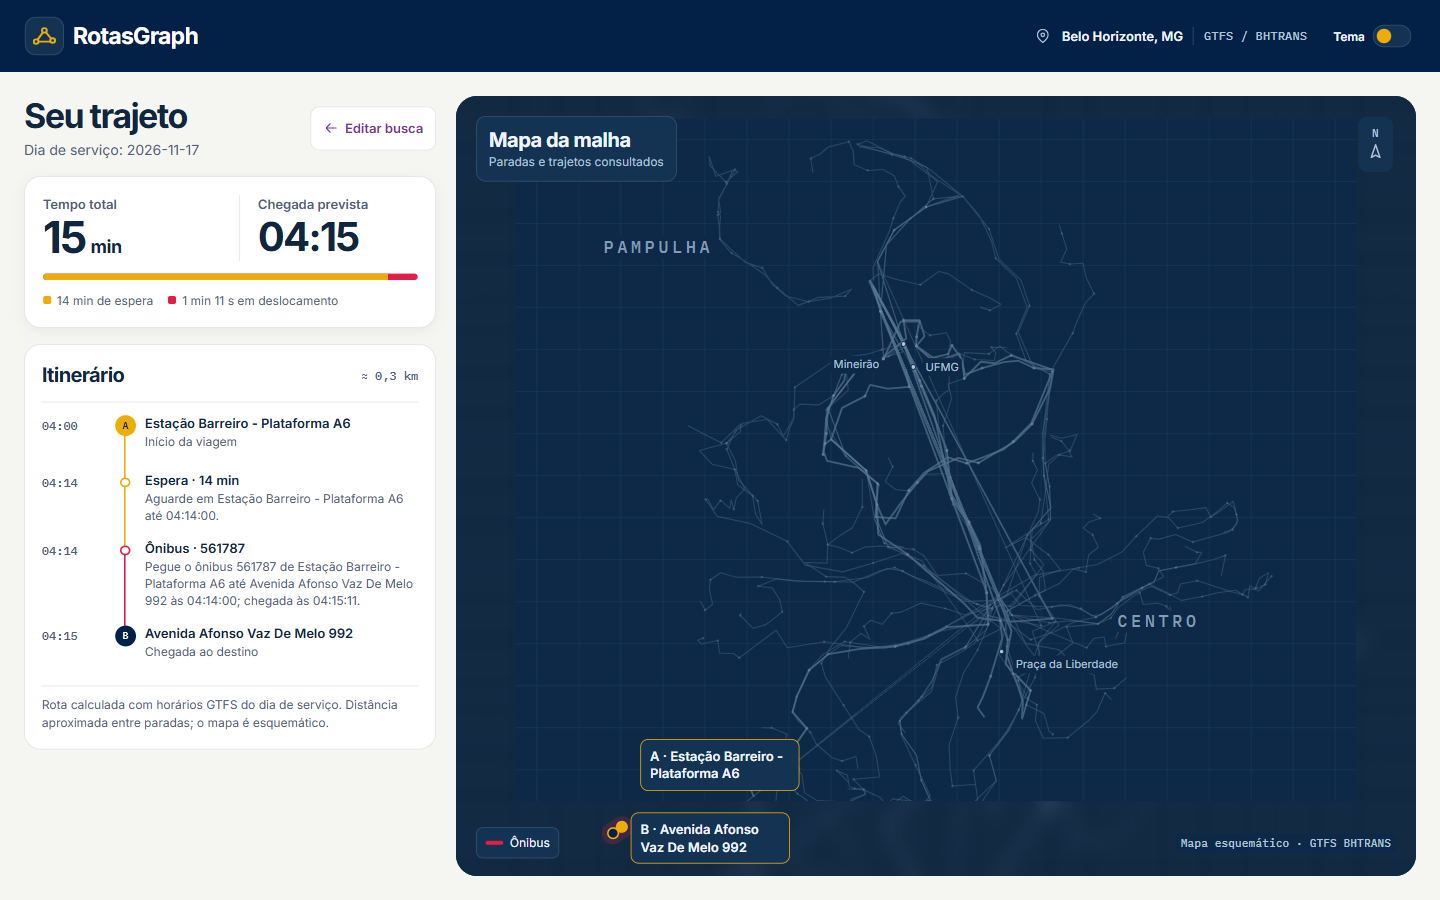
\includegraphics[width=\textwidth]{../../../Artefatos/Prototipos/prototipo-3-instrucoes.png}
\column{.29\textwidth}
\small 17/11/2026\par
15140072 $\rightarrow$ 14788235\par
Partida: 04:00\par\medskip
Chegada: 04:15:11\par
Espera: 14 min\par
Viagem: 1 min 11 s\par
Total: 15 min 11 s\par\medskip
Mapa esquemático e instruções da mesma resposta.
\end{columns}
\end{frame}
% 8:10-9:00 Wanessa
\begin{frame}{Benchmark: preparação, consulta e memória}
\small
54 processos, 384 amostras e 96 resumos; chegadas coincidentes.\par\smallskip
\begin{tabularx}{\textwidth}{@{}Xrr@{}}
\toprule Rede completa & A* nativo & NetworkX \\
\midrule
Preparação mediana (ms) & 734,682 & 14.333,139 \\
RSS preparada mediana (MiB) & 212,301 & 2.237,703 \\
Pico máximo amostrado (MiB) & 228,215 & 2.488,203 \\
\bottomrule
\end{tabularx}
\smallskip
Completo: 6/8 casos com rota; recortes 100/1.000: 0/8.\par\smallskip
Nas consultas, NetworkX teve menor mediana nos seis casos com rota; um caso sem rota inverteu a relação. Representações e condições distintas impedem superioridade geral.
\vfill\tiny Fonte: docs/benchmarks/campaign/full/; sete repetições, dois aquecimentos.
\end{frame}
% 9:00-10:00 Caio e todos
\begin{frame}{O que o MVP demonstra}
\begin{block}{Resultado}
Roteamento de menor chegada com hipóteses explícitas, domínio independente da interface e evidência estrutural reproduzível.
\end{block}
\medskip
Limites: horários planejados, sem trânsito ao vivo, tarifa ou tempo mínimo de transferência.\par\medskip
Evolução: estado de viagem, geometria de ruas e múltiplos dias exigem rever o modelo.\par\medskip
\small Responsabilidades e commits: docs/AUTHORSHIP\_AUDIT.md.\par
Artigo, referências e dados: docs/report/rotasgraph.tex.
\end{frame}
\end{document}
